\section{Introduction}
% introduce the problem you want to solve, expain why it is important to solve it; and indicate the method you used to solve it. add a concept figure showing the overall idea behind the method you are presenting.
\begin{figure*}[h]
    \begin{center}
        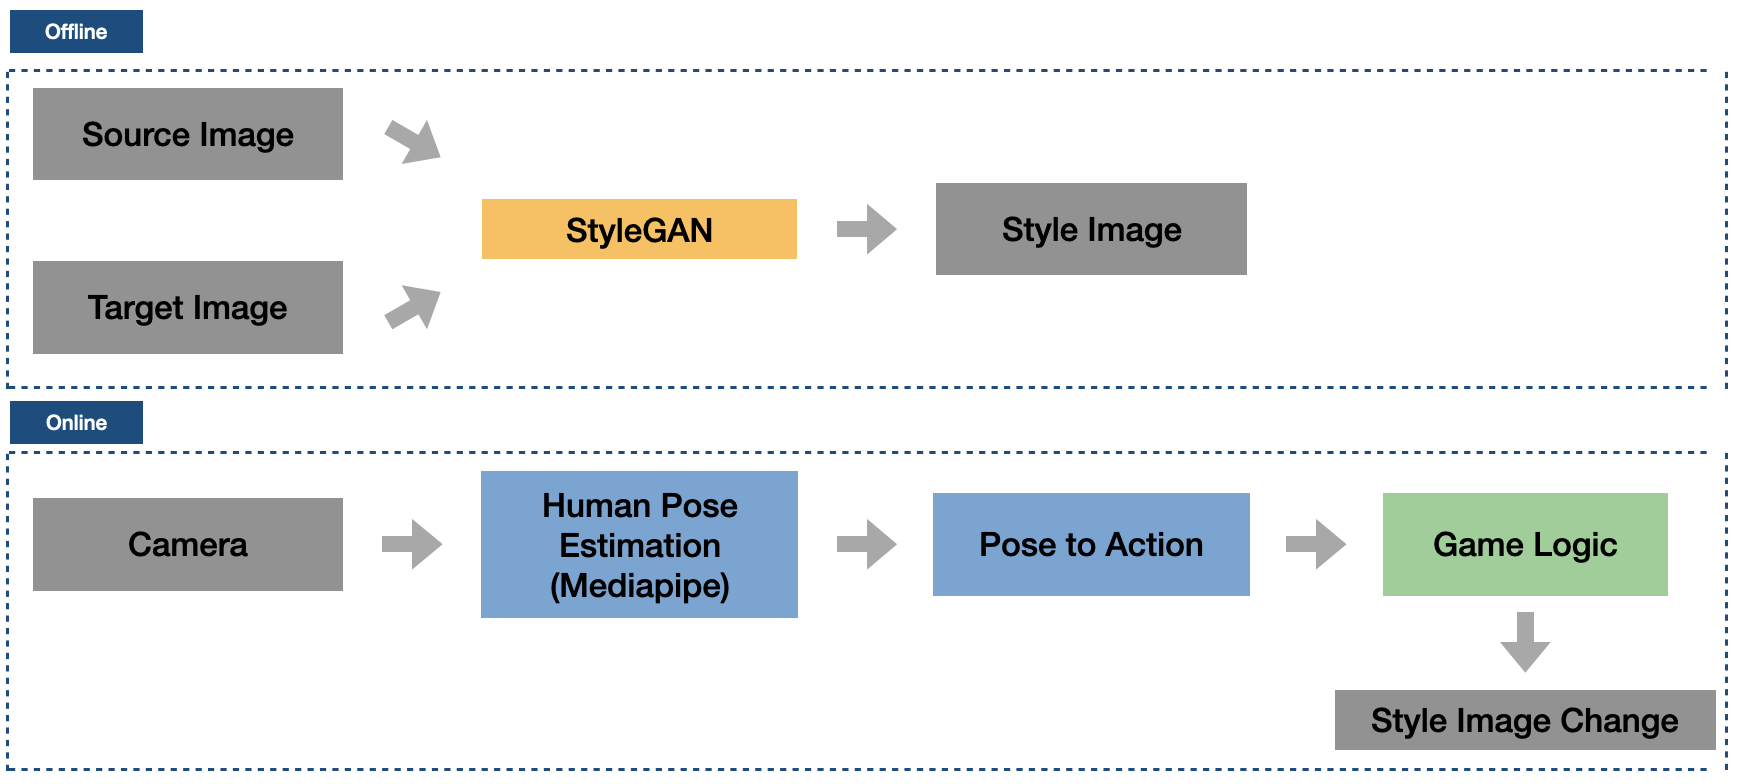
\includegraphics[width=1.0\linewidth]{fig/cv_framework.png}
    \end{center}
    \caption{\textbf{System flow chart} Players will take a selfie respectively as their player avatar before the game starts. During the game, the camera will capture the players’ human pose, reflecting the human pose in the game. The faces in the game will also change by time according to the health points of each player.
    }
    \label{fig:framework}
\end{figure*}
Many computer vision techniques incorporate forms of machine learning and have been applied to various video games, such as Minecraft and Super Mario. These application of computer vision focuse on interpreting game events using visual data.

Based on those existing computer-vision-based games, we develop a two-player fighting game. There are some game rules in the following:
\begin{enumerate}
    \item[(1)] When entering the game, two players will take a selfie respectively as their initial player avatar in the game.
    \item[(2)] The camera will capture the players' human pose, reflecting the human pose in the game. There are five actions defined by the relative positions of key points. For example, when the player raises his/her right hand, the avatar goes right.
    \item[(3)] The players' faces (source face) will change to another face (target face) step by step.
    \item[(4)] The more health points a player loses, the more his/her face will change. 
    \item[(5)] The player should try his/her best in order to keep his/her face from turning into other people's faces.
\end{enumerate}

To achieve the goal above, we use StyleGAN~\cite{karras2019style} to generate a sequence of images that are style mixed between the source face and the target face. For real-time human action detection, we use mediapipe~\cite{lugaresi2019mediapipe} to implement it. To combine these parts into a game, the game logic is needed. 

Our contributions are combining all above elements and implementing into a real-time fighting game without the need of GPU, and achieving excellent performance (some actions even achieve 100\% accuracy) on human action detection.

